%%%%%%%%%%%%%%%%%%%%%%%%%%%%%%%%%%%%%%%%%%%%%%%%%%%%%%%%%%%%%%%%%%%%%%%%%%
%%  CHAPTER 2 -- CARBON LEAKAGE WITHIN AND ACROSS COUNTRIES
%%  ~10 minutes. 5 slides.  (numbers on slides 3 & 4 only)
%%%%%%%%%%%%%%%%%%%%%%%%%%%%%%%%%%%%%%%%%%%%%%%%%%%%%%%%%%%%%%%%%%%%%%%%%%

%%%%%%%%%%%%%%%%%%%%% (1) OVERVIEW %%%%%%%%%%%%%%%%%%%%%%%%%%%%%%%%%%%%%%%%
\begin{frame}{Carbon leakage within and across countries}

    \begin{tcolorbox}[colback=red!4,colframe=red!50!black]
        \textbf{Question:} does the EU ETS push activity toward \emph{less-regulated} suppliers ---
        \alertr{within} Belgium and \alertr{across} its borders?
    \end{tcolorbox}

    \begin{wideitemize}
        \item \textbf{\alertoch{Data:}} firm-level Belgium --- near-universe \alertb{B2B network} $+$ firm$\times$product$\times$country \alertp{customs} $+$ \alertg{EUTL} emissions/allowances
        \item \textbf{\alertb{Approach:}} continuous-treatment DiD --- dose $=$ a supplier's predetermined \alerto{carbon-cost exposure}; shock $=$ the \alerto{2015 MSR}-driven EUA run-up
        \item \textbf{\alertr{Result:}} carbon pricing \alertg{does} raise producer prices (more in exposed sectors) --- but sourcing \alertr{does not move}. \textbf{Three margins, three nulls.}
        \item \textbf{\alertp{Why:}} the relative-price gap stays \alertr{tiny} even at full pass-through --- too small to repay switching
    \end{wideitemize}

\end{frame}

%%%%%%%%%%%%%%%%%%%%% (2) PASS-THROUGH (+ SETTING) %%%%%%%%%%%%%%%%%%%%%%%
\begin{frame}{First: the policy \emph{does} bite on prices}

    \begin{columns}
    \begin{column}{0.55\textwidth}
        \begin{figure}
            \centering
            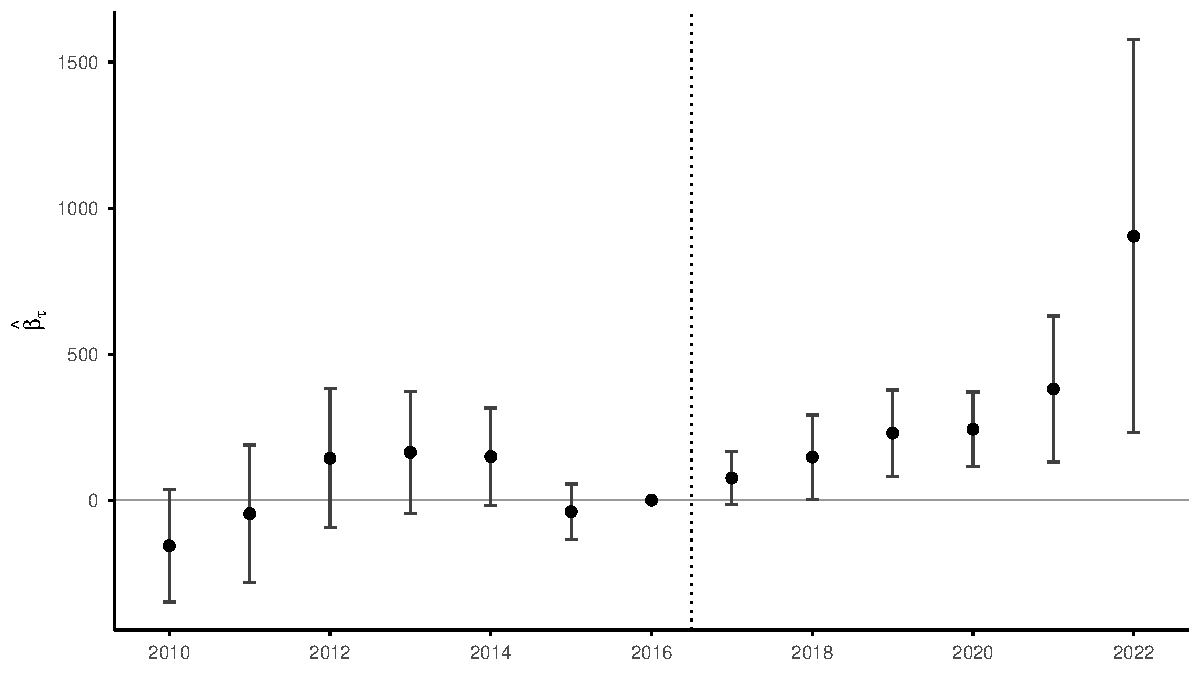
\includegraphics[width=\linewidth]{figures/phase4_ppi_eventstudy_omega_sh.pdf}
        \end{figure}
    \end{column}
    \begin{column}{0.45\textwidth}
        \begin{wideitemize}
            \item \textbf{\alerto{Shock}}: the 2015 MSR drives EUA \alertr{\texteuro5 $\to$ \texteuro80+} --- mechanical, predetermined
            \item \textbf{\alerto{Dose}}: supplier's pre-2017 exposure $\omega = \tfrac{\text{shortage}}{\text{total cost}}$
            \item Manufacturing prices rise after 2017 and \alertg{stay elevated}
            \item Concentrated in \alertb{shortage}-exposed sectors: \alertg{$+0.012^{**}\!\to\!+0.023^{***}$} per SD \\ {\footnotesize (gross emissions: \alertr{null})}
        \end{wideitemize}
    \end{column}
    \end{columns}

\end{frame}

%%%%%%%%%%%%%%%%%%%%% (3) DOMESTIC NULL (+ WHY) %%%%%%%%%%%%%%%%%%%%%%%%%%
\begin{frame}{Margin 1 --- within Belgium: no reallocation}

    \begin{columns}
    \begin{column}{0.55\textwidth}
        \begin{figure}
            \centering
            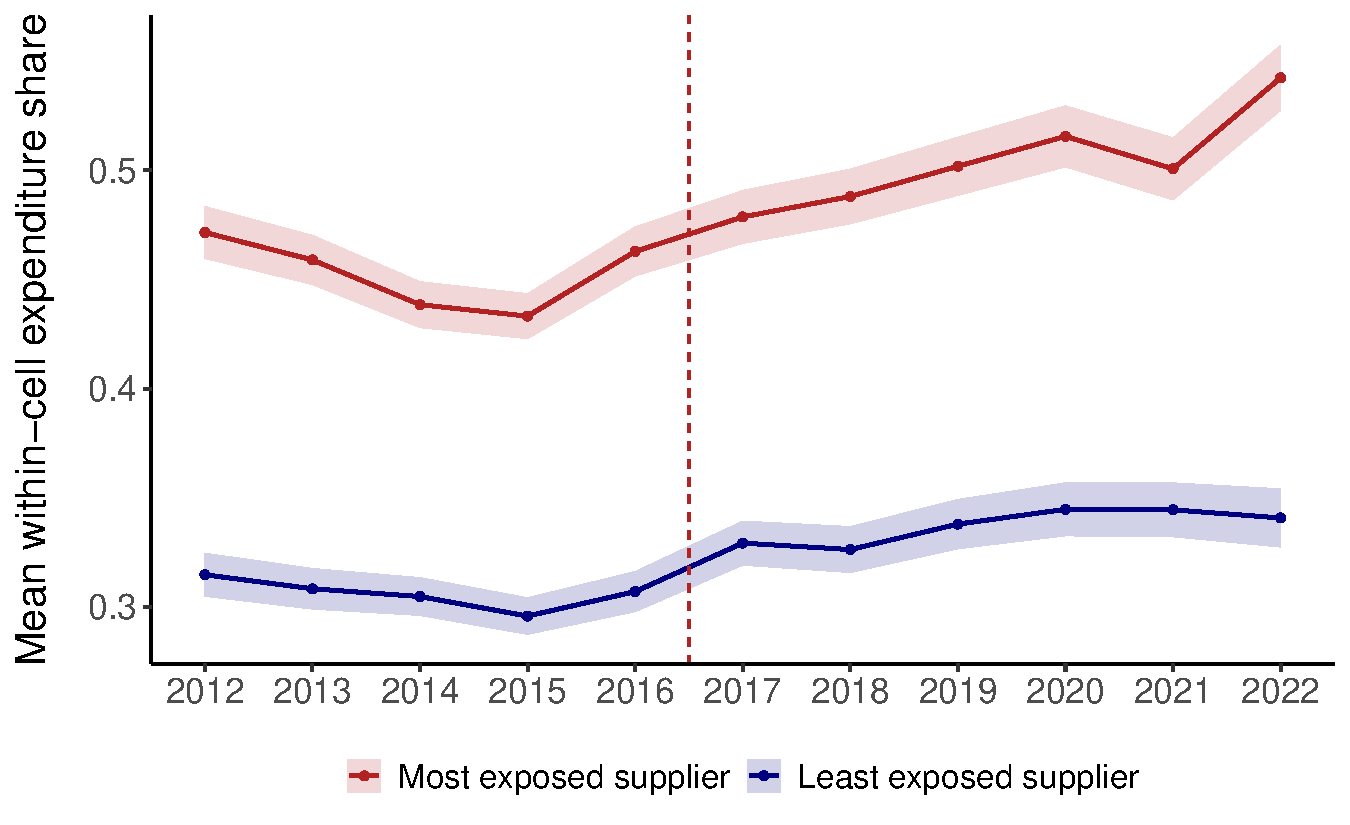
\includegraphics[width=\linewidth]{figures/phase4_within_nace4d_descriptive_trajectory_2017_activeAtT.pdf}
        \end{figure}
    \end{column}
    \begin{column}{0.45\textwidth}
        \begin{wideitemize}
            \item Expenditure share on \alertb{most-} vs.\ \alertr{least-}exposed supplier moves in \alertg{parallel} after 2017
            \item DiD on post$\times$top: \alertr{$+0.0123^{**}$} (wrong sign) $\to$ \alertg{$0.0031$ n.s.} once mechanical attrition is absorbed; not robust under HonestDiD
            \item \textbf{\alertb{Why}}: even at full pass-through the relative-price gap is \alertr{$<1\%$} --- too small to act on
        \end{wideitemize}
    \end{column}
    \end{columns}

\end{frame}

%%%%%%%%%%%%%%%%%%%%% (4) INTERNATIONAL NULL %%%%%%%%%%%%%%%%%%%%%%%%%%%%%
\begin{frame}{Margin 2 --- across borders: Belgium $\neq$ France}

    \begin{columns}
    \begin{column}{0.54\textwidth}
        \begin{figure}
            \centering
            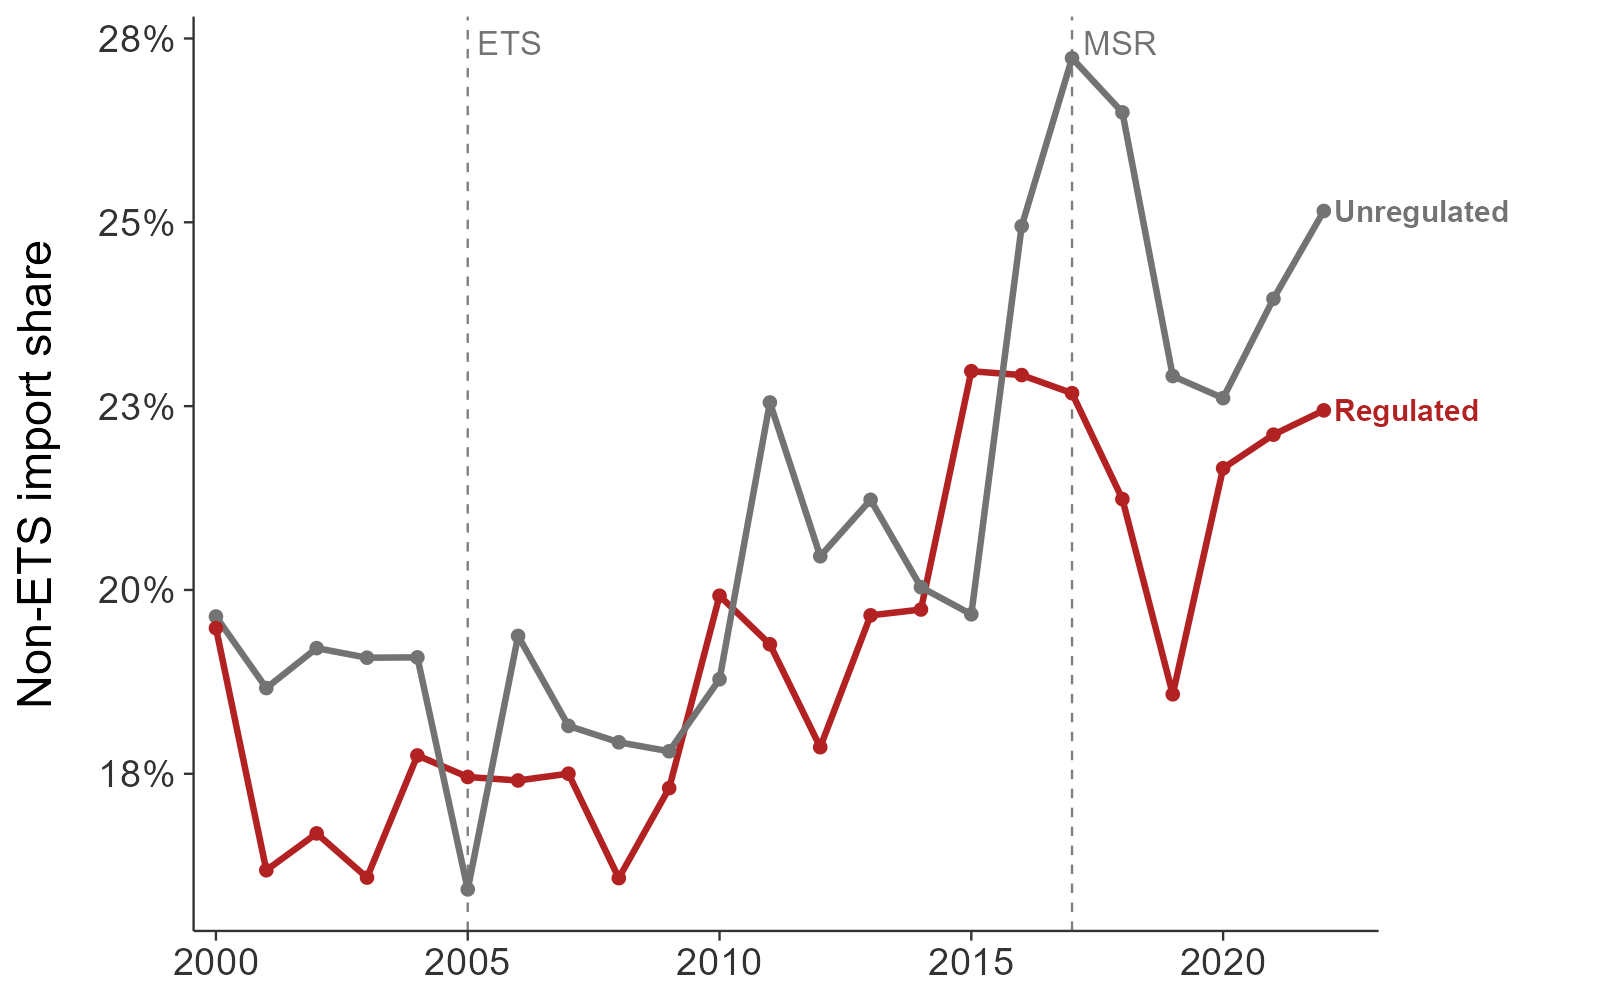
\includegraphics[width=\linewidth]{figures/phase2_cdgm_figure2_share.png}
        \end{figure}
    \end{column}
    \begin{column}{0.46\textwidth}
        \begin{wideitemize}
            \item Replicate Coster--M\'ejean--di Giovanni on Belgian customs: regulated imports, EU vs.\ non-EU sources
            \item Regulated $\times$ non-ETS share is \alertg{flat} across 2000--2022
            \item[] Intensive margin (value share):
            \begin{wideitemize}
                \item[-] Belgium: \alertr{$+0.0004$} (n.s.)
                \item[-] France: \alertb{$+0.121$} ($p<0.001$)
            \end{wideitemize}
            \item[] \alertp{$\Rightarrow$} a common EU carbon price need \alertr{not} produce the same leakage everywhere
        \end{wideitemize}
    \end{column}
    \end{columns}

\end{frame}

%%%%%%%%%%%%%%%%%%%%% (5) TAKEAWAYS %%%%%%%%%%%%%%%%%%%%%%%%%%%%%%%%%%%%%%%
\begin{frame}{Chapter 2 --- three margins, three nulls}

    \begin{tcolorbox}[colback=red!4,colframe=red!50!black]
        \centering The set of margins with detectable leakage is \textbf{empty}.
    \end{tcolorbox}

    \begin{wideitemize}
        \item[\alertg{1.}] Pass-through is \alertg{real} and persistent --- more in shortage-exposed sectors
        \item[\alertr{2.}] \alertr{No} within-NACE reallocation: wrong-signed, shrinks to insignificance, not robust
        \item[\alertr{3.}] \alertr{No} international reallocation: flat shares, far below France
    \end{wideitemize}

    \vspace{0.2cm}
    \alertp{Mechanism}: the cost shock is small and pass-through partial $\Rightarrow$ the relative-price gap never clears the cost of switching suppliers.

    \vspace{0.1cm}
    {\color{dgray}\small $\hookrightarrow$ Chapters 1--2 measure firms and test reallocation \emph{reduced-form};
    Chapter~3 builds the structural model that says \emph{when} reallocation should bind.}

\end{frame}
